\subsection{Anotação Semântica Colaborativa}\label{4-edicacao-semantica-colaborativa}

Por meio do menu de colaboração, um usuário pode compartilhar o seu projeto com outros usuários. Um projeto refere-se às especificações WSDL juntamente com as ontologias OWL abertas na ferramenta. O primeiro passo para o trabalho colaborativo é compartilhar o projeto com outro usuário. Grasews disponibiliza um menu com funcionalidades relacionadas à edição colaborativa. Um usuário de Grasews pode convidar outro usuário para o trabalho colaborativo. O usuário convidado pode ser tanto um novo usuário quanto um usuário já existente. O usuário convidado receberá um \textit{e-mail} que permitirá que ele aceite ou negue o convite para a edição colaborativa. Caso seja um novo usuário e aceite o convite, Grasews solicitará que realize o cadastro na ferramenta. Tendo aceito o convite, após autenticar-se na ferramenta, o usuário poderá abrir a especificação WSDL e as ontologias OWL compartilhadas com ele, da mesma forma como se tivesse sido este usuário que houvesse carregado estes documentos na ferramenta.

Uma vez com a especificação WSDL aberta no sistema, múltiplos usuários podem anotar semanticamente o documento. A partir deste ponto, todo o trabalho realizado é compartilhado e simultaneamente disponibilizado aos demais usuários que estão com a mesma especificação WSDL aberta na ferramenta. Caso haja outros usuários autenticados e com a mesma especificação WSDL aberta na ferramenta, por meio do compartilhamento da especificação, o projeto destes usuários é automaticamente atualizado, trazendo as edições recentemente realizadas na especificação WSDL. Desta forma, o grafo e o menu \textit{tree-view} são automaticamente atualizados de forma a representarem a última versão da especificação WSDL compartilhada. De modo a facilitar o trabalho colaborativo e remoto, Grasews provê um conjunto de notificações que são disparadas aos usuários conforme o trabalho é realizado. Tais notificações aparecem no canto inferior direito da ferramenta.

A \figurename~\ref{fig:grasews-anotacao-semantica-compartilhada} ilustra um caso de uso durante o processo de anotação semântica de forma colaborativa. À esquerda, encontram-se os estados do ambiente de trabalho de um \texttt{Usuário A}, enquanto que à direita encontram-se os ambientes de trabalho de um \texttt{Usuário B}. A \figurename~\ref{fig:grasews-anotacao-semantica-compartilhada}a e a \figurename~\ref{fig:grasews-anotacao-semantica-compartilhada}b ilustram os ambientes de trabalho do \texttt{Usuário A} e do \texttt{Usuário B}, respectivamente, em seus estados iniciais. A \figurename~\ref{fig:grasews-anotacao-semantica-compartilhada}c ilustra o ambiente de trabalho do \texttt{Usuário A} após este ter adicionado um \textit{Model Reference} ao elemento tipo complexo \texttt{MyMethodResponseB}, na lateral direita do grafo. Simultaneamente, a \figurename~\ref{fig:grasews-anotacao-semantica-compartilhada}d ilustra o ambiente de trabalho do \texttt{Usuário B} com o mesmo estado inicial, pois a nova anotação semântica ainda não foi notificada ao \texttt{Usuário B}. A \figurename~\ref{fig:grasews-anotacao-semantica-compartilhada}e ilustra o ambiente de trabalho do \texttt{Usuário A} com a anotação semântica feita anteriormente. Finalmente, a \figurename~\ref{fig:grasews-anotacao-semantica-compartilhada}f ilustra o ambiente de trabalho do \texttt{Usuário B} após receber a notificação e a atualização com a anotação semântica criada pelo \texttt{Usuário A} anteriormente.

%\begin{landscape}
    \begin{figure}[h!]
        %\resizebox{\textwidth}{!}{
            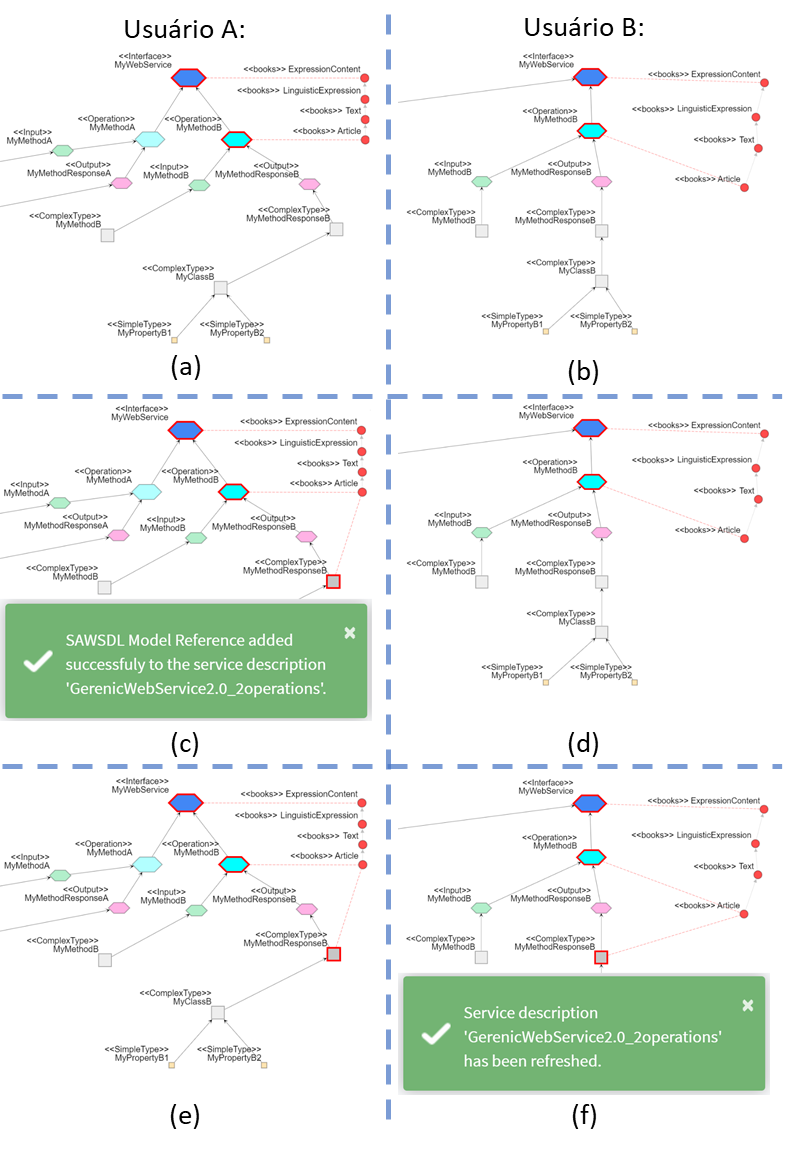
\includegraphics[scale=0.66]{4-grasews/imagens/grasews-anotacao-semantica-compartilhada.png}
        %}
        \centering
        \caption[Processo de anotação semântica de forma colaborativa de Grasews]{\textbf{Processo de anotação semântica de forma colaborativa de Grasews.} (a) Estado inicial de \texttt{Usuário A}. (b) Estado inicial de \texttt{Usuário B}. (c) \texttt{Usuário A} adiciona uma anotação semântica. (d) \texttt{Usuário B} ainda com estado inicial. (e) Estado final de \texttt{Usuário A} com a nova anotação semântica. (f) \texttt{Usuário B} recebe notificação e atualização com a nova anotação semântica.}
        \label{fig:grasews-anotacao-semantica-compartilhada}
    \end{figure}
%\end{landscape}

De forma a evitar inconsistências nas edições colaborativas de uma especificação WSDL, Grasews controla o trabalho colaborativo por meio dos módulos \texttt{Grasews.Application} e \texttt{Grasews.Postgres}. \texttt{Grasews.Application} garante que requisições de anotações semânticas, criadas pelo módulo \texttt{Grasews.API}, sejam verificadas e validadas juntamente com o \texttt{Grasews.Postgres} a fim de que um usuário não sobrescreva o trabalho de outro usuário por conta de requisições concorrentes. Assim, caso haja requisições concorrentes para a anotação de um mesmo elemento WSDL/XSD, apenas a primeira requisição recebida será processada, enquanto que as demais serão descartadas. Todos os usuários que criaram anotações semânticas de forma concorrente recebem notificações da ferramenta com os resultados de suas requisições, sejam os resultados de sucesso ou não. Entretanto, caso requisição seja descartada para um dado usuário, este pode remover anotações que foram realizadas por ele e por outros usuários e, então, adicionar novas anotações na especificação WSDL.

Por fim, cada usuário que possui uma especificação WSDL compartilhada com outros usuário pode reposicionar os nós do grafo individualmente. Grasews permite que cada usuário salve o seu próprio grafo com os ajustes (reposicionamentos) realizados. Este recurso também possibilita que cada usuário possa realizar a anotação semântica de forma personalizada, já que cada usuário pode ter uma forma diferente de compreender do grafo. Entretanto, as anotações realizadas na especificação e, consequentemente, as notações visuais do grafo são automaticamente compartilhadas, independentemente das posições dos nós do grafo. Note que na \figurename~\ref{fig:grasews-anotacao-semantica-compartilhada}, as posições dos nós do grafo do \texttt{Usuário A}, à esquerda, diferem das posições dos nós do grafo do \texttt{Usuário B}, à direita.